\chapter{Felhasználói felület}

\section{Szöveges be- és kimenetek a szimulációhoz}

\subsection{Cél és áttekintés}
A rendszer szöveges alapú beállításra és eredménygyűjtésre alkalmas. 
A cél, hogy a szimuláció \emph{kiegészítő eszközök} (pl.\ curl, CSV-konverzió) nélkül, 
egyszerű szövegfájlokkal legyen vezérelhető és kiértékelhető.

\noindent Rövid összefoglaló:
\begin{itemize}
  \item \textbf{Bemenetek:} \texttt{thresholds.txt}, \texttt{esp\{1..3\}\_schedule.txt}, \texttt{sim\_control.txt}
  \item \textbf{Kimenet/napló:} \texttt{output.txt} (idősoros; egy sor = egy vezérlési ciklus)
  \item \textbf{Webes felület:} ``Dev Panel'' (localhost:8080) a fájlok szerkesztéséhez, generálásához, 
  letöltéséhez, a futás indításához/megállításához, az idő nullázásához és a napló törléséhez.
\end{itemize}

\subsection{Bemeneti szövegfájlok}

\subsubsection{\texttt{thresholds.txt} -- küszöbök és maximum megengedhető áram}
A vezérlő szerver minden ciklusban beolvassa. Kulcs--érték párok, tizedes ponttal:
\begin{verbatim}
# Küszöbértékek a vezérlő szerverhez
BREAKER_MAX_TOTAL=65.0    # [A] - Megszakító lekapcsolási áram
BREAKER_MIN_TOTAL=35.0    # [A] - Megszakító bekapcsolási áram
ALLOC_MAX_TOTAL=95.0      # [A] - Max áram érték
\end{verbatim}

\noindent Megjegyzések:
\begin{itemize}
  \item A \emph{megszakítók} (breakerek) logikája az \emph{aktuálisan mért hatásos} összáramhoz 
  viszonyít (\texttt{BREAKER\_MAX\_TOTAL}, \texttt{BREAKER\_MIN\_TOTAL}).
  \item A SIM-ekre küldött korlátok (cap) a \emph{nyers igényekből} számítódnak \emph{max-min fair} elv 
  szerint, az \texttt{ALLOC\_MAX\_TOTAL} keret figyelembevételével.
\end{itemize}

\subsubsection{\texttt{esp\{x\}\_schedule.txt} -- idősoros bemenet}
Formátum: időpillanat másodpercben + kívánt áram (A). A menetrend \emph{lépcsős}: a legutóbbi időponthoz 
tartozó érték érvényes a következő megadásig.
\begin{verbatim}
# seconds  amps
0         1.0
30        2.5
120       0.8
\end{verbatim}
\noindent Irányelvek: tizedes elválasztó pont; tetszőleges szóköz; a sorok idő 
szerint rendezve mint minden szöveges ki- és bemeneti file-ban.

\subsubsection{\texttt{sim\_control.txt} -- futtatási állapot}
Egyetlen szó: \texttt{RUNNING} vagy \texttt{STOPPED} (Az alapértelmezés \texttt{STOPPED}). 
A SIM-ek ``virtuális órája'' csak \texttt{RUNNING} állapotban megy.

\subsection{Kimeneti szövegfájl}

\subsubsection{\texttt{output.txt} -- idősoros kimenet}
A vezérlő minden ciklusban \emph{egy sort} ír. A fájl alapértelmezetten \emph{append-only} 
a véletlen szerkesztést elkerülendő; a Dev Panel ``Clear output.txt'' művelete törli amennyiben ez szükséges, 
és a vezérlő legközelebb automatikusan újra létrehozza a fejlécet.

\noindent Formátum: \texttt{kulcs=érték} párok szóközzel elválasztva.
\begin{verbatim}
# One record per line; fields are key=value separated by spaces
timestamp=1758199200 sim_state=RUNNING sum_current_amps=5.7 \
alloc_max_total_amps=6.0 max_total_amps=6.0 min_total_amps=1.0 \
sims=esp1:raw=2.0,effective=2.0,cap=2.0|esp2:raw=1.7,effective=1.7,
cap=2.0|esp3:raw=2.5,effective=2.0,cap=2.0 \
breakers=brk1:on,brk2:on
\end{verbatim}

\noindent Kulcsok a kimeneti file-ban:
\begin{itemize}
  \item \texttt{timestamp} -- UNIX időpecsét (s).
  \item \texttt{sim\_state} -- globális állapot: \texttt{RUNNING}/\texttt{STOPPED}.
  \item \texttt{sum\_current\_amps} -- mért hatásos összáram (cap után).
  \item \texttt{alloc\_max\_total\_amps} -- allokációs keret (A).
  \item \texttt{max\_total\_amps} / \texttt{min\_total\_amps} -- breaker küszöbök (legacy nevek).
  \item \texttt{sims} -- \texttt{|} jellel szeparált lista SIM-enként:\\
  \texttt{espX:raw=\dots, effective=\dots, cap=\dots}\\
  ahol \texttt{raw} = menetrendi igény, \texttt{effective} = tényleges áram, \texttt{cap} = küldött maximum.
  \item \texttt{breakers} -- megszakítók állapota \texttt{on}/\texttt{off}, vesszővel elválasztva.
\end{itemize}

\subsection{Időkezelés és futtatás}
\begin{itemize}
  \item \textbf{Virtuális idő:} minden SIM saját menetrendi ideje csak \texttt{RUNNING} állapotban növekszik.
  \item \textbf{STOPPED} módban a SIM-ek ideje megáll; a vezérlő nem küld új cap-et és 
  nem kapcsolgat megszakítót, csak mér és naplóz.
  \item \textbf{Reset (t=0):} a Dev Panel ``Reset sim time (t=0)'' gombja az összes 
  SIM virtuális idejét nullázza (a panel előbb STOP-ra állít, majd resetel).
\end{itemize}

\subsection{Reprodukálhatóság és feldolgozhatóság}
A bemenetek (küszöbök, menetrendek, futtatási állapot) verziózhatók és mellékelhetők. 
A kimeneti \texttt{output.txt} önleíró; minden rekord tartalmazza az adott ciklus lényeges paramétereit. 
A formátum egyszerűen feldolgozható bármely nyelven (kulcs=érték párok; \texttt{sims} és \texttt{breakers} 
mezők jól definiált szeparátorokkal).

\subsection{Rövid példa -- beállítás $\rightarrow$ kimenet (részlet)}

\paragraph{thresholds.txt}
\begin{verbatim}
BREAKER_MAX_TOTAL=9.0
BREAKER_MIN_TOTAL=2.0
ALLOC_MAX_TOTAL=9.0
\end{verbatim}

\paragraph{esp1\_schedule.txt}
\begin{verbatim}
# seconds  amps
0  50
60 10
\end{verbatim}

\paragraph{esp2\_schedule.txt}
\begin{verbatim}
0  50
60 10
\end{verbatim}

\paragraph{esp3\_schedule.txt}
\begin{verbatim}
0  50
60 100
\end{verbatim}

\noindent Várható kiosztás a 0--60 s szakaszban: mindhárom SIM korlátozott, 
mivel az igény 150 A $>$ 9 A. 60 s után az 
igények \texttt{[10, 10, 100]} $\Rightarrow$ kiosztás \texttt{[10, 10, 70]}. A \texttt{cap} és 
az \texttt{effective} értékek ennek megfelelően jelennek meg az \texttt{output.txt}-ben.

% =====================================================================
\chapter{Max--min fair (water-filling) elosztás}

\section{Elméleti háttér és cél}

\subsection{Motiváció és cél}
A szimulált fogyasztók  áramigénye (\(d_i\)) időben változik. 
Adott egy globális, maximum áramérték \(\,B=\texttt{ALLOC\_MAX\_TOTAL}\,\) amperben, 
ennél a tényleges összáram nem lehet nagyobb. A cél egy olyan kiosztás \(\,a_i\) meghatározása, amely
(i) nem lépi túl az egyes igényeket (\(0\le a_i\le d_i\)),
(ii) a teljes kereten belül marad (\(\sum_i a_i \le B\)),
(iii) és \emph{fair} a kis igényűekkel szemben, azaz a kis igények teljesülnek először, a 
fennmaradó kapacitás pedig egyenlő alapról oszlik meg.

\subsection{Definíció (max--min fair)}
Egy \(\,a=(a_1,\dots,a_n)\) kiosztás \emph{max--min fair}, ha bármely más megengedett \(\,y\) esetén, 
ha létezik \(i\) úgy, hogy \(y_i > a_i\), akkor létezik \(j\) olyan, hogy \(a_j \le a_i\) és \(y_j < a_j\). 
Intuíció: csak a \emph{már kisebb} részesedésűek rovására lehet növelni bárki juttatását. \cite{wiki:max-min-fairness}

\subsection{Feltöltés (water-filling)}
A max--min fair kiosztás felírható egyetlen paraméterrel:
\begin{equation}
  a_i = \min\{\,d_i,\ \lambda\,\}, \qquad \text{ahol }\ \sum_{i=1}^n \min\{d_i,\lambda\} \;=\; B.
\end{equation}
A \(\lambda\) \emph{vízszint} úgy választandó, hogy a keret pont kiteljen (vagy ha \( \sum_i d_i < B\), 
akkor \(\lambda\ge \max_i d_i\), vagyis nincs korlát).

\subsection{Algoritmus és bonyolultság}
Gyakorlati, determinisztikus eljárás (progresszív töltés):
\begin{enumerate}
  \item Rendezzük az igényeket növekvő sorrendbe: \(d_{(1)} \le \dots \le d_{(n)}\).
  \item Iteráljuk \(k=1..n\): feltételezzük, hogy az első \(k\) igény teljesül (\(a_{(i)}=d_{(i)}\), \(i\le k\)), 
  és a maradék \(B_k = B - \sum_{i=1}^k d_{(i)}\) egyenlő szinten oszlik meg a még nyitott \(n-k\) elemre. 
  A jelölt vízszint: \(\lambda_k = B_k/(n-k)\).
  \item Ha \(\lambda_k \le d_{(k+1)}\), megtaláltuk a vízszintet: az összes hátralévő \(a_{(i)}=\lambda_k\) 
  (és a korábbiak \(d_{(i)}\)).
  \item Ha minden \(d_{(i)}\) teljesül és még marad keret, akkor nincs korlátozás: \(a_i=d_i\).
\end{enumerate}
A rendezés miatt az időbonyolultság \(O(n\log n)\). A megvalósított vezérlőben egy ekvivalens, 
iteratív \emph{progresszív} algoritmus fut, amely kis elemszámon szintén gyors és stabil.

\begin{figure}
    \centering
    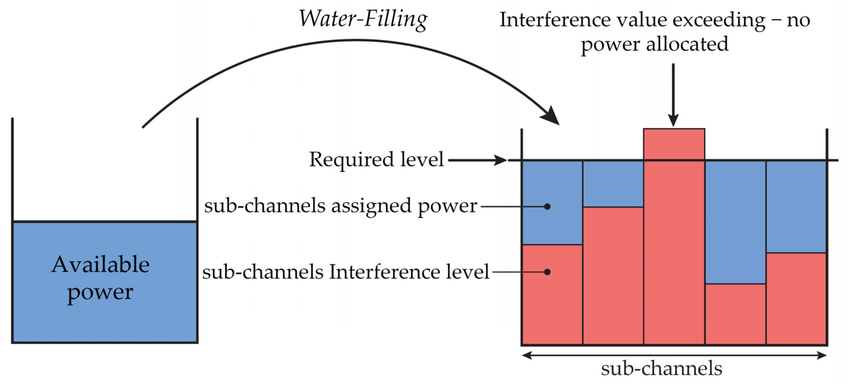
\includegraphics[width=1\textwidth]{figures/Principle-of-Water-Filling-algorithm-76.png}
    \caption{Water-filling elve telekomunikációban. \cite{Slacik2021Sensors}}
    \label{fig:water-filling}
\end{figure}

\subsection{Tulajdonságok}
\begin{itemize}
  \item \textbf{Egyenlő szint elve:} a \(\lambda\) alatti igények teljes, a \(\lambda\) 
  felettiek \(\lambda\)-ig kapnak. Így a kis igényűek sosem szenvednek hátrányt.
  \item \textbf{Monotonitás:} ha a keret \(B\) nő, akkor \(\lambda\) nem csökken, és senki kiosztása nem csökken.
  \item \textbf{Határhelyzetek:} ha \(\sum_i d_i \le B\) → nincs cap (végtelen korlát). Ha \(B=0\) → minden \(a_i=0\).
\end{itemize}

\section{A vezérlőben alkalmazott megvalósítás}

\subsection{Kapcsolat a rendszer komponenseivel}
A vezérlő igényekből (\texttt{raw\_current}) számolja a limiteket a fenti elv szerint 
a \texttt{ALLOC\_MAX\_TOTAL} kereten. A \emph{megszakító} (breaker) logika ettől független, 
a \emph{mért, tényleges} áramhoz viszonyít (\texttt{BREAKER\_MAX\_TOTAL}, \texttt{BREAKER\_MIN\_TOTAL}) 
biztonsági rétegként.

\subsection{Példák}
\paragraph{Klasszikus példa.}
\(d=[10,10,100]\), \(B=90\) \(\Rightarrow\) \(a=[10,10,70]\) (a két kicsi teljesül, a maradék egy szinten oszlik meg).
\paragraph{Vegyes igények.}
\(d=[3,8,8,20]\), \(B=25\) \(\Rightarrow\) rendezve az első igény (3) teljesül, a maradék \(22\) 
három felé oszlik: \(a=[3,\,7.33,\,7.33,\,7.33]\) A.

\subsection{Implementációs részletek}
A limitek csak \(\pm 10^{-3}\) A változás felett frissülnek a fogyasztók felé (zajcsillapítás), 
a „nincs korlát” állapotot nagy \(\texttt{INF\_CAP}\) érték reprezentálja. Ha a nyers igény összeg a keret alá esik, 
a limitek feloldódnak.

% =====================================================================

\chapter{Fejlesztői panel (Dev Panel)}

\section{Cél és szerep}
A Dev Panel egy könnyű használatú webes felület, amely a szöveges bemenetek és kimenetek kezelését, 
a futtatás indítását/megállítását, az idő nullázását és a napló törlését teszi lehetővé. Célja 
a \emph{gyors kísérletezés} és a \emph{reprodukálható} tesztfutások támogatása külön eszközök nélkül.

\section{Architektúra áttekintése}
A panel egy Flask-alapú backendből (\texttt{/api/*}) és statikus frontendből (HTML+CSS+JS) áll. 
A backend közvetlenül a \texttt{./data} mappában található fájlokat kezeli, 
és hálózaton hívja az esp-t szimuláló konténerek végpontjait. A vezérlő külön, 
a saját portján (\(8000\)) fut; a Prometheus és Grafana eléréséhez gyorslinkek állnak rendelkezésre.

\section{Fő funkciók és munkamenet}
\paragraph{Start/Stop.} A \texttt{sim\_control.txt} fájlba írja a panel 
a \texttt{RUNNING} vagy \texttt{STOPPED} értéket. STOP módban az esp szimulátorok virtuális ideje megáll, 
a vezérlő nem küld max értékeket és nem kapcsol megszakítókat, csak mérést és naplózást végez.
\paragraph{Reset (t=0).} A panel a STOP beállítás után meghívja minden esp szimulátor \texttt{/reset\_time} 
végpontját, a virtuális idejük nulláról indul újra.
\paragraph{Clear output.txt.} A \texttt{data/output.txt} törlése. A vezérlő a következő ciklusban 
automatikusan újra létrehozza a fejlécet és folytatja a naplózást.
\paragraph{Thresholds szerkesztés.} A \texttt{thresholds.txt} beolvasása/írása a panelről: 
\texttt{BREAKER\_MAX\_TOTAL}, \texttt{BREAKER\_MIN\_TOTAL}, \texttt{ALLOC\_MAX\_TOTAL}.
\paragraph{Menetrend-generátor.} Konstans, fel- és lefutás, lépcső, szinusz és random walk idősorok képezhetők 
a \texttt{esp\{x\}\_schedule.txt} fájlokba (formátum: \texttt{seconds\ \ \ amps}). 
A generált tartalom előnézetben ellenőrizhető.
\paragraph{Raw editor \& Letöltés.} Tetszőleges bemeneti fájl közvetlen szerkeszthető; 
az \texttt{output.txt} csak olvasható. Minden be- és a kimenet letölthető megőrzéshez.

\section{Backend API (elérések)}
\begin{center}
\begin{tabular}{ll}
\hline
\textbf{Végpont} & \textbf{Funkció} \\
\hline
\texttt{GET\ /api/read?name=...} & Fájl beolvasása \\
\texttt{POST\ /api/write} & Fájl írása \\
\texttt{GET\ /api/download?name=...} & Közvetlen letöltés \\
\texttt{GET\ /api/sim\_state} & Globális állapot lekérdezése \\
\texttt{POST\ /api/sim\_state} & RUNNING/STOPPED beállítása \\
\texttt{POST\ /api/clear\_output} & \texttt{output.txt} törlése \\
\texttt{POST\ /api/reset\_sim\_time} & Minden szimulátor időnullázása \\
\hline
\end{tabular}
\end{center}

\section{Biztonsági és korlátok}
A panel \emph{belső} használatra készült. Nincs többfelhasználós jogosultság- és CSRF-kezelés; 
éles környezetben ezeket pótolni szükséges. A fájlműveletek engedélyezett listához kötöttek, 
a végpontok nem tesznek lehetővé tetszőleges fájlhozzáférést.

\section{Kiterjeszthetőség}
A panel könnyen bővíthető új be- és kimenetekkel: pl.\ súlyozott fair-elosztás bemenete (\texttt{weights.txt}), 
előre definiált menetrend-sablonok, vagy beépített grafikon a \texttt{output.txt} vizualizálására. 
A funkcionalitás változtatása különösen egyszerű, mivel az állapot \emph{szöveges fájlokban} 
van deklarálva.

\begin{figure}
    \centering
    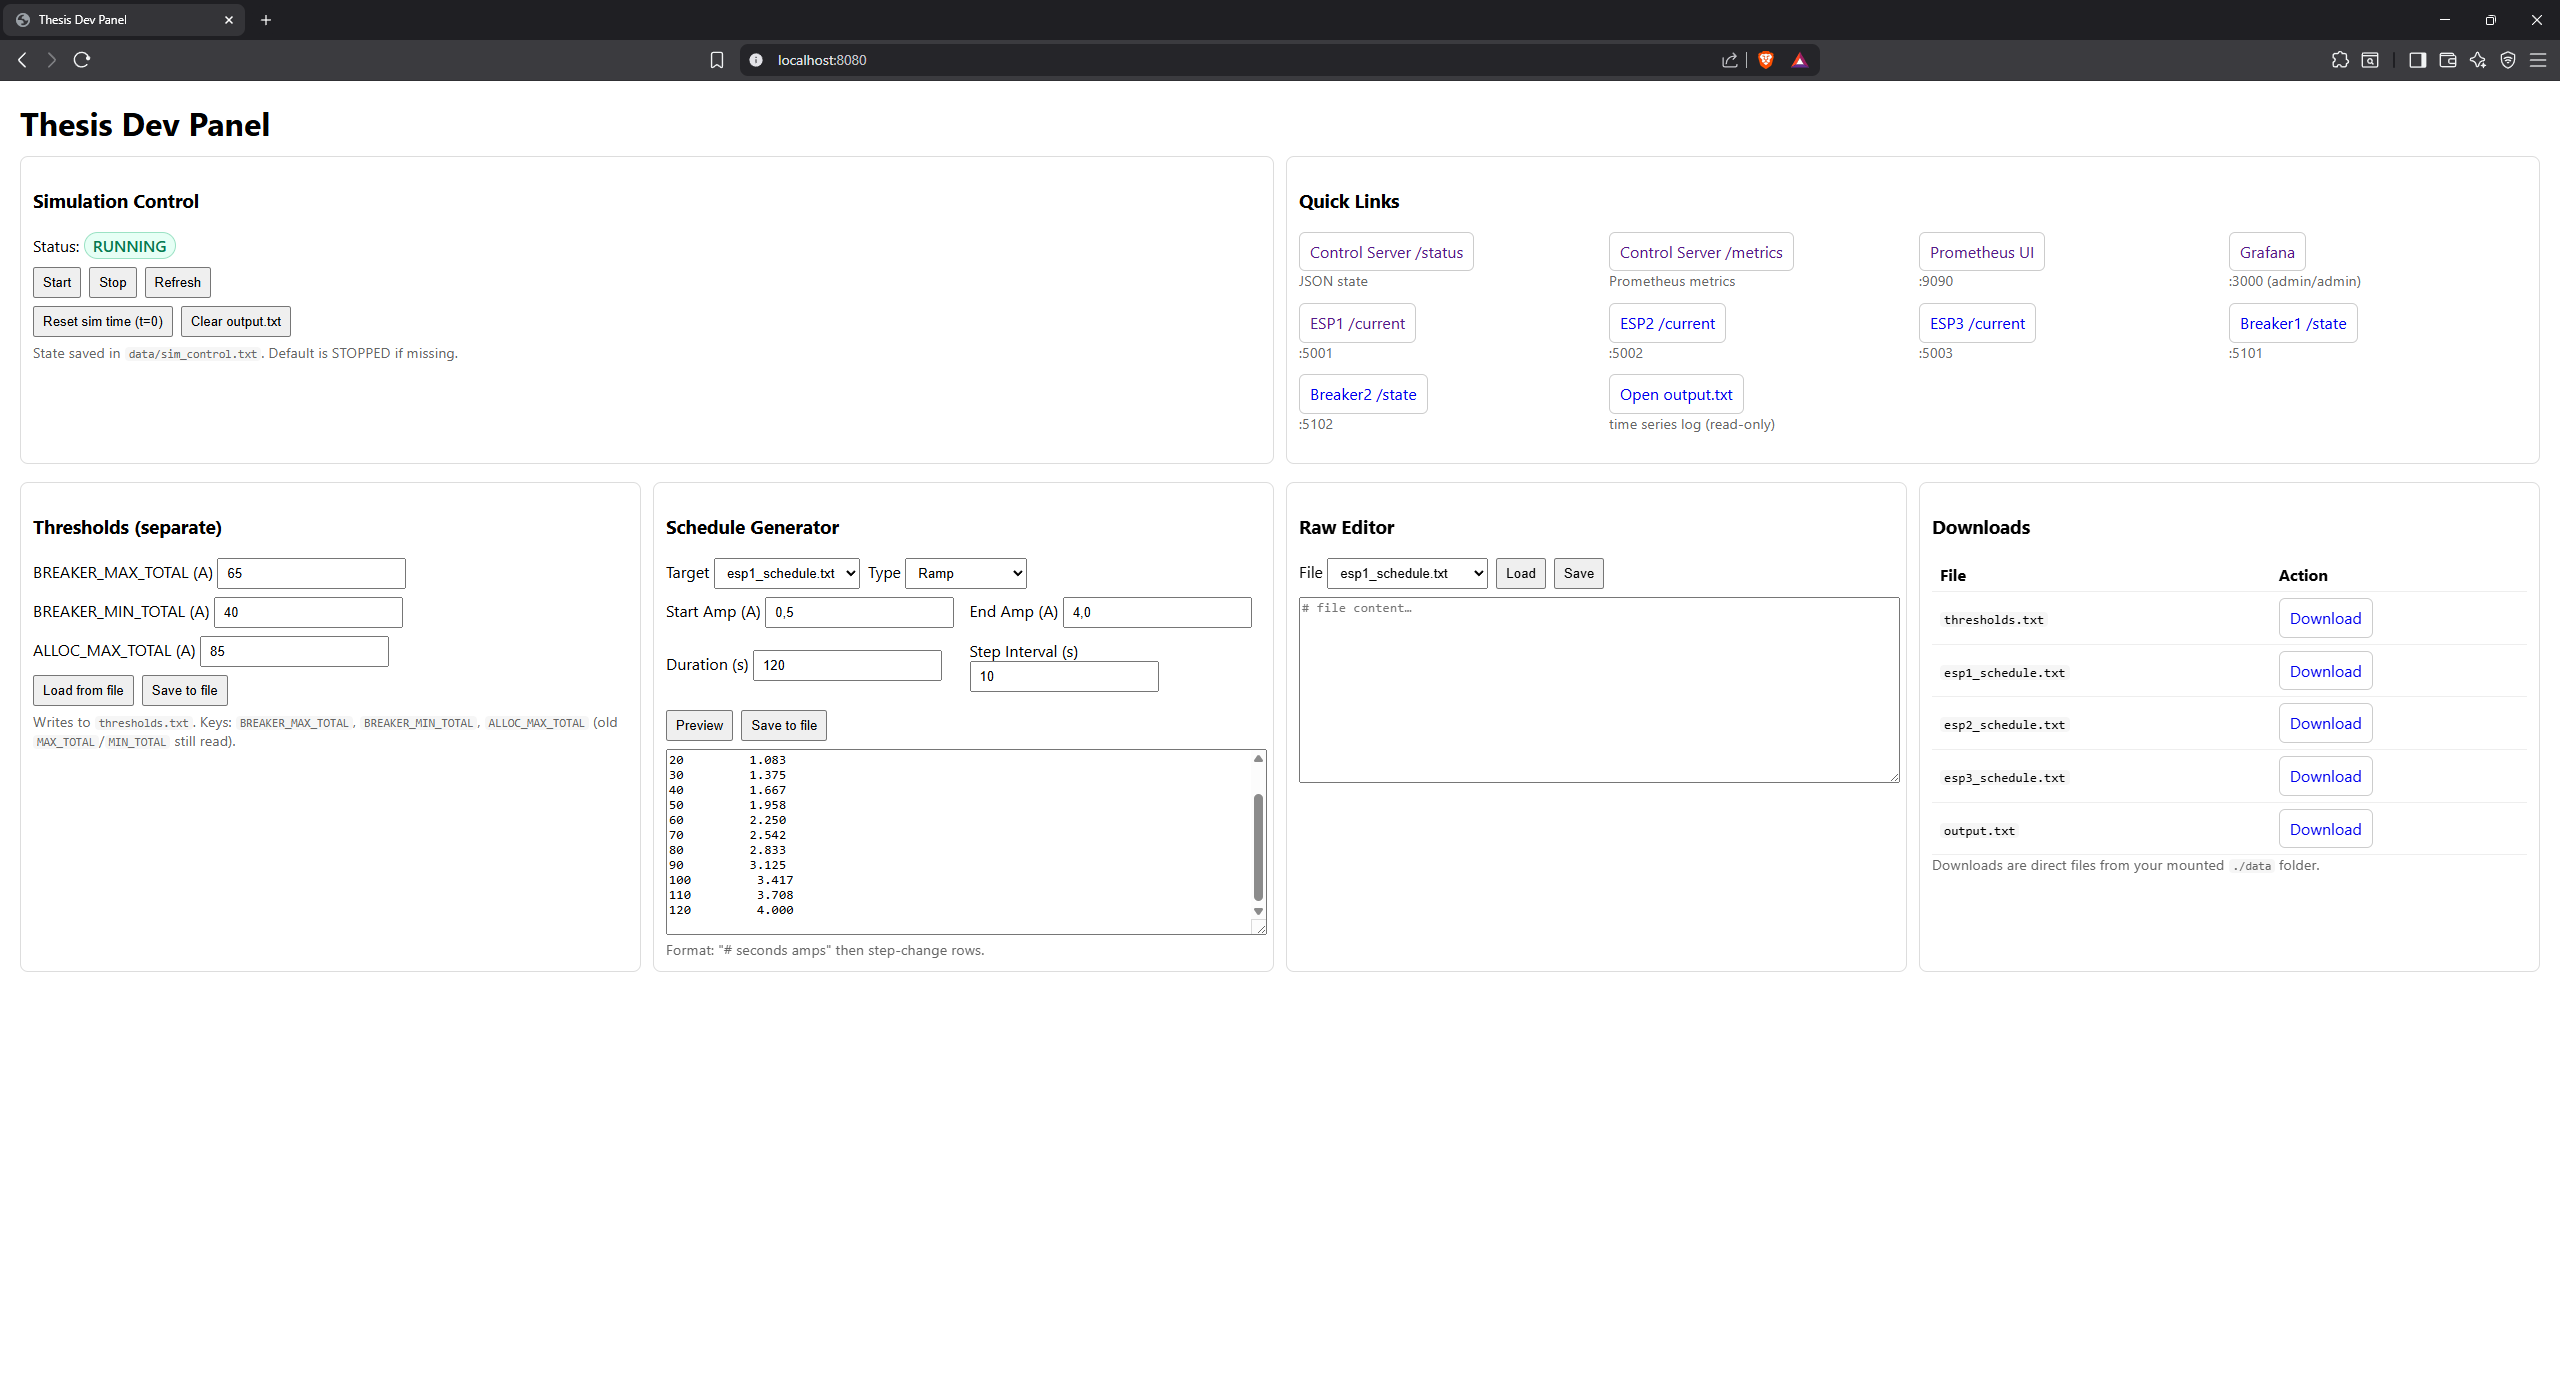
\includegraphics[width=1\textwidth]{figures/devpanel.png}
    \caption{Devpanel}
    \label{fig:devpanel}
\end{figure}